\section{Method}
\label{sec:method}
\begin{figure}[!t]
\centering
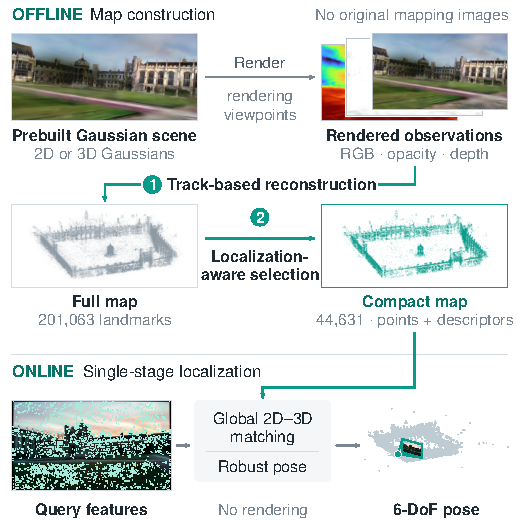
\includegraphics[width=\linewidth]{Fig2_overview.pdf}
\caption{Offline map construction and online localization. Rendered reference views provide observations for track reconstruction and compact-map selection. The deployed map stores coordinates and descriptors; a real query is localized by direct 2D--3D matching and robust pose estimation. Default map construction requires no original mapping images.}
\label{fig:fig2}
\end{figure}


Given a prebuilt Gaussian scene, AnyGSLoc constructs an explicit landmark map offline and then removes the renderer from the localization path. The construction follows the dependency of the information itself: rendered reference observations are first made reliable and associated into tracks; each track is then converted into a 3D landmark with a descriptor and uncertainty; finally, the candidate landmarks are selected according to their value for localization. Figure~\ref{fig:fig2} gives the complete pipeline. Thus, tracks provide the correspondence evidence, reconstruction turns that evidence into localization landmarks, and selection determines which landmarks need to be deployed.

\subsection{Problem Formulation and Map Representation}
\label{sec:overview}

Let a prebuilt Gaussian scene be $\mathcal G$. We choose reference cameras $\{(K_m,R_m,t_m)\}_{m=1}^{M}$ and render RGB $I_m$, opacity $\alpha_m$, and depth $Z_m$. Poses map world coordinates to camera coordinates, so the camera center is $C_m=-R_m^\mathsf Tt_m$ and the image projection is $\pi_m(X)=\operatorname{proj}(K_m(R_mX+t_m))$, where $\operatorname{proj}$ denotes perspective division. These cameras are rendering viewpoints and need not coincide with the original mapping cameras. The default pipeline uses rendered observations; the optional use of original mapping images is evaluated in Sec.~\ref{sec:input-availability}.

A localization landmark should represent one repeatedly observed image feature. Let $\mathcal T_i$ contain the observation indices $(m,k)$ belonging to landmark $i$, and let $\mathcal W_i$ be its supporting reference views. The reconstruction stage produces
\begin{equation}
\begin{aligned}
\mathcal A&=\{(X_i,d_i,\mathcal T_i,q_i,\Sigma_i^X)\}_{i=1}^{N},\\
\mathcal M_S&=\{(X_i,d_i):i\in S\},\qquad S\subseteq\{1,\ldots,N\}.
\end{aligned}
\label{eq:landmark}
\end{equation}
Here $X_i\in\mathbb R^3$ and the unit descriptor $d_i\in\mathbb R^{D_f}$ are the deployed landmark attributes. The scalar quality $q_i$ and approximate position covariance $\Sigma_i^X$ guide offline selection. We call $\mathcal A$ the \emph{Full} candidate bank and $\mathcal M_S$ the \emph{Compact} map. After export, localization needs only these landmark records and their search index; the Gaussian scene is no longer queried.

\subsection{Track Construction from Rendered Observations}
\label{sec:observations}
\label{sec:construction}
\begin{figure*}[t]
\centering
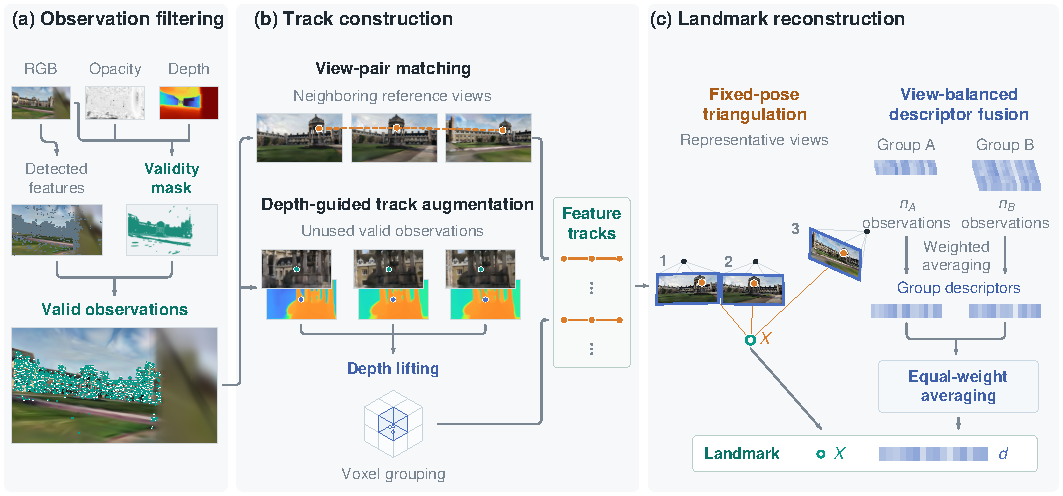
\includegraphics[width=\linewidth]{Fig3_reconstruction.pdf}
\caption{Rendering-aware landmark construction. (a) Observation filtering combines rendered RGB structure, opacity, and depth into a validity mask before cross-view association. (b) View-pair matching and depth-guided augmentation form geometrically verified tracks. (c) Fixed-pose triangulation estimates coordinates; view-balanced aggregation forms one descriptor per track. The example tracks use the MAtCha configuration evaluated in Table~\ref{tab:t8}.}
\label{fig:fig3}
\end{figure*}


The first stage determines which rendered detections should be treated as observations of the same scene feature. A strong detector response is not sufficient: rendering artifacts or weakly supported regions can yield distinctive but unreliable observations. We therefore filter detections before association and use calibrated epipolar geometry to verify the correspondences that form each track.

\paragraph{Observation filtering}
Frozen SuperPoint~\cite{detone2018superpoint} detects features on the complete rendered RGB image. For detection $o_{mk}=(u_{mk},d_{mk},s_{mk})$, $u_{mk}$ is the image coordinate, $d_{mk}$ is its unit descriptor, and $s_{mk}$ is its detector score. We evaluate three complementary validity tests at the detection location: geometric support $v_m^{\rm geom}$ from opacity and depth, local appearance support $v_m^{\rm app}$ from image structure, and region validity $v_m^{\rm reg}$ for unreliable image regions. Their conjunction defines the observations admitted to cross-view association:
\begin{equation}
\begin{aligned}
v_m(u)&=v_m^{\rm geom}(u)v_m^{\rm app}(u)v_m^{\rm reg}(u),\\
\mathcal O_m&=\{o_{mk}:v_m(u_{mk})=1\}.
\end{aligned}
\label{eq:observation_filter}
\end{equation}
The filter is applied after feature extraction and therefore controls the observations entering association rather than modifying the image seen by SuperPoint.

\paragraph{Geometrically verified tracks}
The retained observations are associated over a sparse graph of neighboring reference cameras. Descriptor similarity proposes candidate matches, while calibrated epipolar geometry rejects incompatible pairs; reciprocity and similarity margins further suppress ambiguous associations. Each accepted edge receives a confidence combining descriptor agreement, epipolar consistency, and detector support. The observation confidence $\gamma_{mi}$ is taken from the strongest accepted incident edge in the primary graph.

We merge accepted edges into tracks in confidence order, giving precedence to associations supported by three-view cycles over isolated chains. A merge is rejected if it would assign two detections from the same camera to one track. Consequently, each track contains at least three views and tracks have disjoint observation ownership. The notation $u_{mi}$, $d_{mi}$, and $s_{mi}$ is therefore unambiguous for $m\in\mathcal W_i$.

\paragraph{Depth-guided track augmentation}
The sparse camera graph does not necessarily connect every useful observation. For unmatched valid detections, rendered depth supplies a coarse world-space location that narrows the search for compatible associations. Candidate matches are then checked by descriptor similarity and epipolar consistency, producing additional tracks under the same one-observation-per-camera and disjoint-ownership constraints. Depth is used here to augment correspondence discovery, not to define the exported coordinate; both association paths feed the same track-based reconstruction in Fig.~\ref{fig:fig3}(b).

\subsection{Track-Based Landmark Reconstruction}
\label{sec:geometry}

A track supplies multiple image measurements of one scene feature. The reconstruction stage turns those measurements into the attributes required by the localization map: a 3D coordinate, a descriptor, and evidence for later selection. The key geometric choice is to let the matched pixels determine the coordinate. A Gaussian center is tied to a rendering primitive, whereas rendered depth provides a view-dependent distance estimate. Neither is guaranteed to be the point that best explains the feature correspondence. We therefore reconstruct the landmark from the calibrated rays associated with its track (Fig.~\ref{fig:fig3}(c)).

\paragraph{Robust multiview triangulation}
Let $\bar u_{mi}$ denote the homogeneous pixel-center coordinate of observation $u_{mi}$. Its unit world bearing is
$r_{mi}=\operatorname{normalize}(R_m^\mathsf TK_m^{-1}\bar u_{mi})$,
and $P_{mi}=I_3-r_{mi}r_{mi}^\mathsf T$ projects onto the plane orthogonal to that bearing. We retain a confidence-ranked geometry subset $\mathcal V_i\subseteq\mathcal W_i$ and estimate the point by minimizing its weighted ray distances:
\begin{equation}
X_i(w)=\arg\min_X\sum_{m\in\mathcal V_i}w_{mi}\lVert P_{mi}(X-C_m)\rVert^2.
\label{eq:triangulation}
\end{equation}
For fixed nonnegative weights, the solution satisfies
\begin{equation}
\begin{aligned}
A_i(w)X_i(w)&=b_i(w),\\
A_i(w)&=\sum_{m\in\mathcal V_i}w_{mi}P_{mi},\\
b_i(w)&=\sum_{m\in\mathcal V_i}w_{mi}P_{mi}C_m.
\end{aligned}
\label{eq:raynormal}
\end{equation}
Thus the coordinate is determined by the calibrated image observations. When the retained bearings are nondegenerate, the normal matrix is positive definite and the estimate is unique~\cite{hartley2004mvg}.

Associations can still contain individual outliers, so we refine the point by reweighting observations according to their reprojection residuals. Let $\bar\gamma_{mi}$ be the normalized base confidence, $z_{mi}^{(t)}$ the camera depth of the current estimate, and $e_{mi}^{(t)}=\lVert\pi_m(X_i^{(t)})-\bar u_{mi,1:2}\rVert_2$ the image residual. Starting from $X_i^{(0)}=X_i(w^{(0)})$ with $w_{mi}^{(0)}=\bar\gamma_{mi}$, each update is
\begin{equation}
\begin{aligned}
w_{mi}^{(t+1)}&=\bar\gamma_{mi}\,\mathbf 1[z_{mi}^{(t)}>0]\,
h_\delta(e_{mi}^{(t)}),\\
X_i^{(t+1)}&=X_i(w^{(t+1)}).
\end{aligned}
\label{eq:rayreweight}
\end{equation}
where $h_\delta(e)=\min\{1,\delta/\max(e,\epsilon)\}$ is a bounded decreasing residual weight. The cameras remain fixed throughout: only the observation weights change, and every update solves the same ray least-squares problem. The final finite, nondegenerate support set is denoted $\mathcal V_i^+$.

\paragraph{View-balanced descriptor fusion}
The track also provides the appearance evidence that will be stored with the reconstructed point. A flat average over all observations would implicitly weight a landmark by the sampling density of its reference views. We instead aggregate observations within pose groups and then give the occupied groups equal influence. For each group $\mathcal C_g$,
\begin{equation}
p_{ig}=\operatorname{normalize}\left(
\sum_{m\in\mathcal W_i\cap\mathcal C_g}a_{mi}d_{mi}
\right),
\label{eq:group_descriptor}
\end{equation}
where $a_{mi}$ combines detector and association confidence. We identify the group descriptor most representative of the others and retain a consistent subset of nearby group descriptors; let $\mathcal K_i$ denote their indices. The exported descriptor is
\begin{equation}
d_i=\operatorname{normalize}\left(
\sum_{g\in\mathcal K_i}p_{ig}
\right).
\label{eq:descriptor}
\end{equation}
This separates observation confidence from view-sampling density: confidence controls aggregation within a group, whereas equal group weights prevent repeated sampling of similar viewpoints from dominating the descriptor. Group-level trimming also limits inconsistent appearance, while deployment stores only one descriptor per landmark.

\paragraph{Quality and geometric uncertainty}
Selection needs two different kinds of evidence: whether a track is reliable and how strongly its position is constrained. Let $\bar e_i$ be the median reprojection residual over $\mathcal V_i^+$ and let $\theta_i$ denote a robust measure of track parallax. We define
\begin{equation}
\begin{aligned}
q_i&=\operatorname{clip}_{[0,1]}\left(q_i^{\rm geom}q_i^{\rm assoc}\right),\\
q_i^{\rm geom}&=\exp(-\bar e_i/\tau_e)
\min\left\{\theta_i/\tau_\theta,1\right\}.
\end{aligned}
\label{eq:landmark_quality}
\end{equation}
The association factor summarizes descriptor agreement and, for primary tracks, edge confidence, view-group support, and cycle evidence. Its exact aggregation and fallback rules are implementation details in Sec.~\ref{sec:implementation}; descriptor agreement used for quality is computed from the track mean independently of the exported group-balanced descriptor.

A scalar score does not reveal directional uncertainty. For example, a narrow-baseline track can have a small reprojection residual while remaining weakly constrained along depth. Let $J_{X,mi}=\left.\partial\pi_m(X)/\partial X\right|_{X_i}$ be the $2\times3$ point-projection Jacobian. Conditional on fixed cameras and associations, we approximate
\begin{equation}
\Sigma_i^X=\widehat\sigma_i^2
\left(\sum_{m\in\mathcal V_i^+}\widehat w_{mi}
J_{X,mi}^{\mathsf T}J_{X,mi}\right)^{-1},
\label{eq:pointcov}
\end{equation}
where $\widehat w_{mi}$ are evaluated at the final estimate and $\widehat\sigma_i^2$ is a robust residual scale. This covariance captures the anisotropy of the reconstructed point and is later propagated into the pose-information model.

\subsection{Localization-Aware Landmark Selection}
\label{sec:selection}
\begin{figure*}[t]
\centering
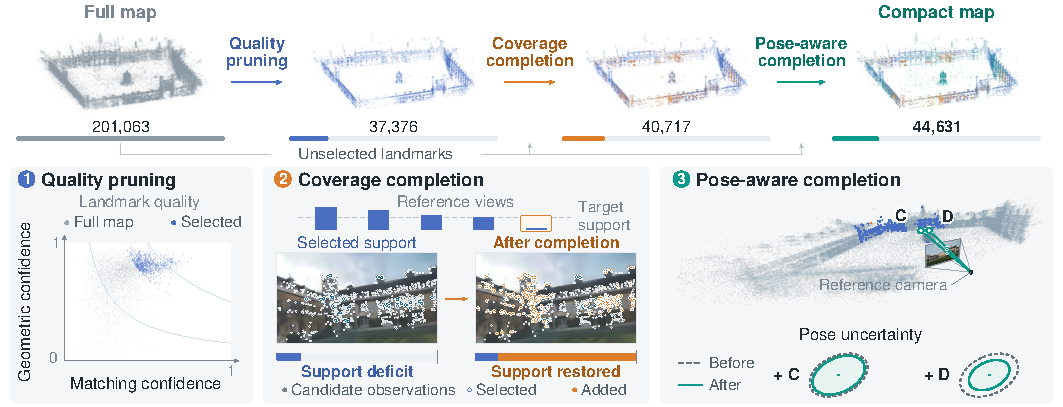
\includegraphics[width=\linewidth]{Fig4_selection.pdf}
\caption{Localization-aware selection on the Great Court 3DGS map. Quality pruning and coverage completion retain 37,376 and 40,717 points. Pose completion adds 4,096 points and cleanup removes 182, leaving 44,631. The lower panels illustrate quality, coverage, and complementary pose constraints; contour changes are emphasized for visibility.}
\label{fig:fig4}
\end{figure*}


The candidate bank is richer than the map that needs to be deployed. Selection therefore asks a different question from reconstruction: not whether a landmark is valid, but whether retaining it adds useful localization support. A quality-only ranking favors strong individual points but can leave some reference views weakly supported; coverage alone can fill those views with redundant points. We therefore proceed in three stages: establish a reliable quality core, restore deficient reference-view support, and add landmarks that contribute complementary local pose information. The final stage also removes coverage-only landmarks that have become redundant. Figure~\ref{fig:fig4} and Algorithm~\ref{alg:selection} summarize the process.

\paragraph{Quality pruning and coverage completion}
For a selected set $S$, define the support of reference view $m$ and the coverage objective by
\begin{equation}
\begin{aligned}
r_m(S)&=\sum_{i\in S}\mathbf 1[m\in\mathcal W_i],\\
b_m&=\min\{b,r_m(\{1,\ldots,N\})\},\\
F_{\rm cov}(S)&=\sum_{m=1}^{M}\omega_m\min\{r_m(S),b_m\}.
\end{aligned}
\label{eq:matchobjective}
\end{equation}
Because observation ownership is disjoint, $r_m(S)$ counts distinct selected features in view $m$. The target $b_m$ prevents the selector from demanding support unavailable in the Full bank, while $\omega_m$ balances reference-camera groups.

Quality pruning initializes $S$ with a quality-ranked prefix until the core support criterion is met. Coverage completion then adds the candidate with the largest marginal increase in $F_{\rm cov}$, directing additions toward views that remain below their targets. These coverage additions are recorded because some may become redundant after pose-aware completion.

\paragraph{Pose-aware completion}
Once basic coverage is available, candidates should be judged by the pose constraints they add to the current map. We linearize projection at each reference camera using a left pose perturbation $\delta\xi=(\delta t^\mathsf T,\delta\theta^\mathsf T)^\mathsf T$. Let $J_{\xi,mi}$ be the corresponding $2\times6$ projection Jacobian and define $\widetilde J_{mi}=J_{\xi,mi}D$, where $D=\operatorname{diag}(s_tI_3,s_rI_3)$ fixes the relative translation and rotation scales. The point Jacobian above propagates landmark uncertainty into the image plane:
\begin{equation}
\begin{aligned}
\Sigma^u_{mi}&=\sigma_{\rm pix}^2I_2+
J_{X,mi}\Sigma_i^XJ_{X,mi}^{\mathsf T},\\
B_{mi}&=q_{mi}\widetilde J_{mi}^{\mathsf T}
(\Sigma^u_{mi})^{-1}\widetilde J_{mi},\\
H_m(S)&=\lambda I_6+
\sum_{i\in S:\,m\in\mathcal W_i}B_{mi}.
\end{aligned}
\label{eq:information}
\end{equation}
The weight $q_{mi}$ combines landmark quality with observation support, while the covariance term attenuates uncertain landmark locations. Candidate contributions $B_{mi}$ are computed before selection; $H_m(S)$ records the information supplied by the landmarks already retained.

We rank an unselected landmark by its conditional information gain:
\begin{equation}
G_i(S)=\sum_{m\in\mathcal W_i}\left[
\log\frac{\det(H_m(S)+B_{mi})}{\det H_m(S)}
+\beta h_{mi}(S)
\right].
\label{eq:posegain}
\end{equation}
The log-determinant term measures the reduction in local pose-uncertainty volume and therefore favors constraints in directions that remain weakly observed. The diversity term $h_{mi}(S)$ rewards categories not yet represented by the selected map. After each accepted landmark, the information matrices and occupied categories are updated, so each candidate is evaluated relative to the map already built.

Pose completion also absorbs the final redundancy cleanup. We revisit only the landmarks introduced during coverage completion and remove one when its affected views still meet the support level attained at the start of cleanup. The targets remain fixed during deletion, so pose-added landmarks can replace redundant coverage-only points without altering the quality core or pose additions. Selection changes only which rows of $\mathcal A$ are retained; the reconstructed coordinates and descriptors are never modified.

\par\medskip
\noindent\begin{minipage}{\linewidth}
\refstepcounter{anygsalgorithm}\label{alg:selection}
\hrule\smallskip
\textbf{Algorithm \theanygsalgorithm. Localization-aware landmark selection}
\smallskip\hrule\smallskip
\small
\textbf{Input:} Candidate bank $\mathcal A$, target support $b$, and selection settings.\\[2pt]
\textbf{1. Quality pruning.} Retain a quality-ranked prefix in $S$ until the core stopping criterion is met.\\[2pt]
\textbf{2. Coverage completion.} While feasible deficits remain, add the candidate with largest positive marginal gain in $F_{\rm cov}$. Record these additions as $\mathcal U_{\rm cov}$.\\[2pt]
\textbf{3. Pose-aware completion.} Add admissible candidates using refreshed $G_i(S)$, updating the information matrices and occupied categories until a stopping criterion is met.\\[2pt]
\hspace*{1em}\emph{Final cleanup:} Freeze $\tau_m=\min\{b,r_m(S)\}$. Visit $\mathcal U_{\rm cov}$ in increasing quality; remove a point only if all affected views retain $\tau_m$.\\[2pt]
\textbf{Output:} $\mathcal M_S=\{(X_i,d_i):i\in S\}$.
\smallskip\hrule
\end{minipage}
\par\medskip


\subsection{Single-Stage Query Localization}
\label{sec:localization}

The exported map is directly compatible with a structure-based localizer. We extract query features with the same frozen SuperPoint encoder, match each query descriptor to the highest-similarity landmark descriptor, and pass the retained correspondences to a single PoseLib call with robust estimation and local optimization~\cite{poselib,fischler1981ransac}. Matching and solver details are fixed in Sec.~\ref{sec:implementation}. No image retrieval, Gaussian rendering, or separate dense refinement is required online.

For $K$ query descriptors, exhaustive descriptor search requires $O(K|S|D_f)$ arithmetic, while the stored coordinate--descriptor arrays contain $(3+D_f)|S|$ values. Map selection therefore reduces both the persistent landmark representation and the number of descriptor comparisons while preserving the same online localization procedure.